\section*{Приложение А}
\addcontentsline{toc}{section}{Приложение А}
\label{sec:Appendix_1} \index{Appendix_1}
\large

\begin{figure}[ht]
\centering 
    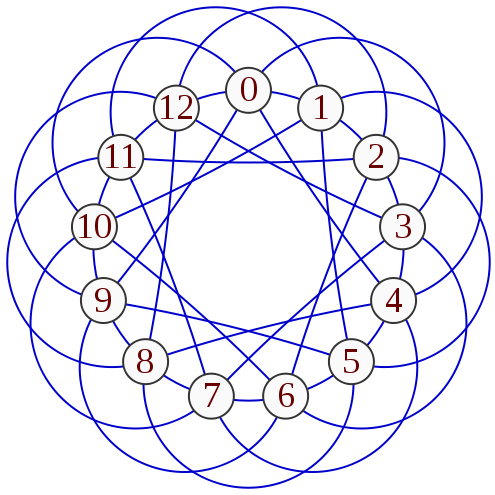
\includegraphics[scale=0.7]{image/srg_example.png}
    \caption{Граф Пейли 13-го порядка, сильно регулярный граф с параметрами srg(13,6,2,3).}
    \label{srg}
\end{figure}

\begin{figure}[H]
\centering
    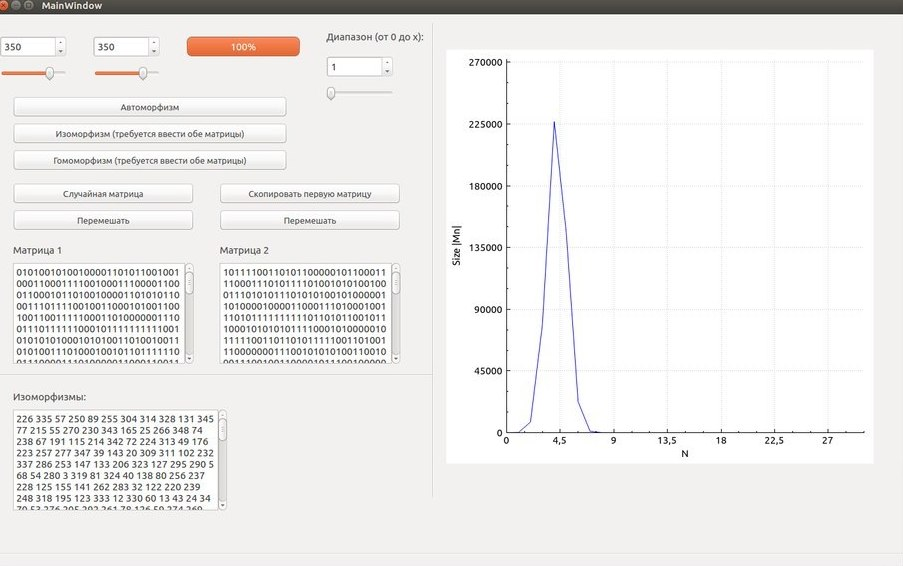
\includegraphics[scale=0.5]{image/program_example.jpeg}
    \caption{Примеры использования программы}
    \label{program_example}
\end{figure}


\begin{figure}[H]
\centering
    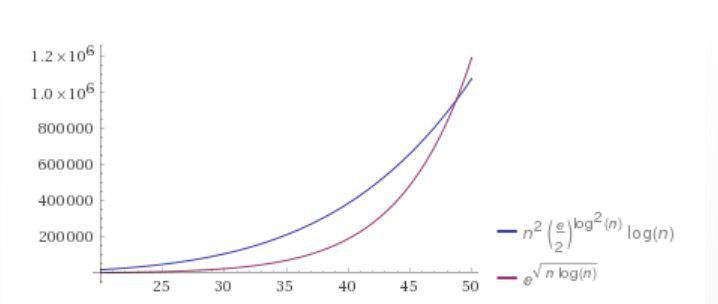
\includegraphics[scale=0.9]{image/graphs.jpg}
    \caption{График сложности алгоритма}
    \label{graphs_func}
\end{figure}

\begin{figure}[H]
\centering
	  \begin{tikzpicture}[domain=1:15, yscale=0.4, xscale=0.7] 
      \draw[step=3, very thin,color=gray] (-0.5,-0.5) grid (15.5,46.5);
      \draw[->] (0,0) -- (16,0) node[right] {$n$}; 
      \draw[->] (0,0) -- (0,47) node[above] {$f(n)$};
      \draw[color=red]    plot (\x,{pow(\x, 2) * pow(e/2, pow(ln(\x), 2)) * ln(\x)/300 })             node[right] {\Large $f(n) = n^2(\frac{e}{2})^{\ln(n)^2} \ln(n)$}; 
      \draw[color=blue]   plot (\x,{pow(e, sqrt(\x * log10(\x)))/20})    node[right] {\Large $f(n) = e^{\sqrt{n \times \log(n)}}$}; 
      \draw[color=blue] plot (\x,{pow(\x, pow(\x ,1/3) * pow(log10(\x), 2))/300}) node[right] {\Large $f(n) = n^{{n^{1/3}\log^{2} n}}$};
  	\end{tikzpicture}
	\caption{График сложности алгоритма}
	\label{algo_func}
\end{figure}


